\newpage
\chapter{Разширени графични възможности и вероятностни разпределения}
\label{chapter08}

\section{Разширени графични възможности}

Към базовите графични възможности на R, пакетите ggplot2 и lattice добавят множество допълнителни възможности. Синтаксисът на извикванията леко се различава от този на функциите в базовите възможности, но това създава затруднения само в началния етап от употребата на двата пакета. 

За визуализация, чрез ggplot2 като основа се използва функцията ggplot. В общия случай тази функция получава, като входен параметър данните за визуализиране и понякога някои допълнителни параметри. Резултатът от изпълнението на ggplot е обект, който в последствие може да бъде допълнително променян, чрез добавяне на възможности с помощта на операцията събиране (+). 

\subsection{Хистограми и плътности}

Хистограмата служи за групиране на стойностите и изброяване на това колко стойности попадат по определените групи. Размерът на всяка група (bin) определя ширината на стълба. 

\begin{lstlisting}[caption=Хистограма и плътност, label=listing0150]
library(ggplot2)

ggplot(data=diamonds) + geom_histogram(aes(x=carat))

ggplot(data=diamonds) + geom_density(aes(x=carat),fill="grey50")
\end{lstlisting}

Както и в предходния пример за хистограма, тук също е представено разпределението на диамантите по карати (Листинг \ref{listing0150}).

\begin{figure}[h!]
  \centering
  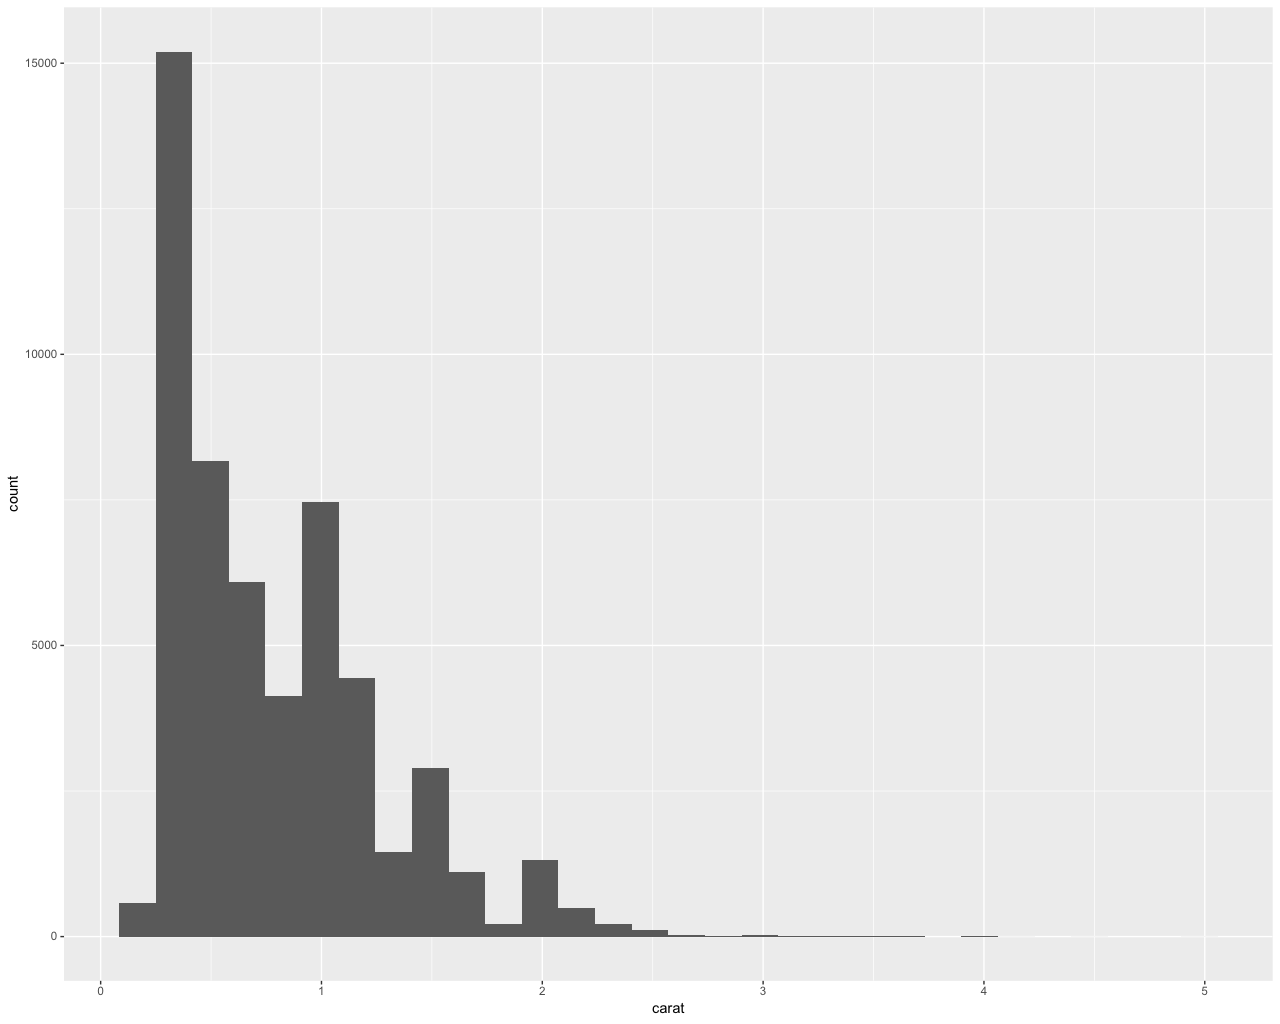
\includegraphics[width=1.0\linewidth]{pic0030}
  \caption{Хистограма при 30 групи}
\label{figure0030}
\end{figure}
\FloatBarrier

Функцията aes определя кои данни да бъдат използвани за разполагане по осите. В примера с диамантите, това е характеристиката за тегло (карат). 

\begin{figure}[h!]
  \centering
  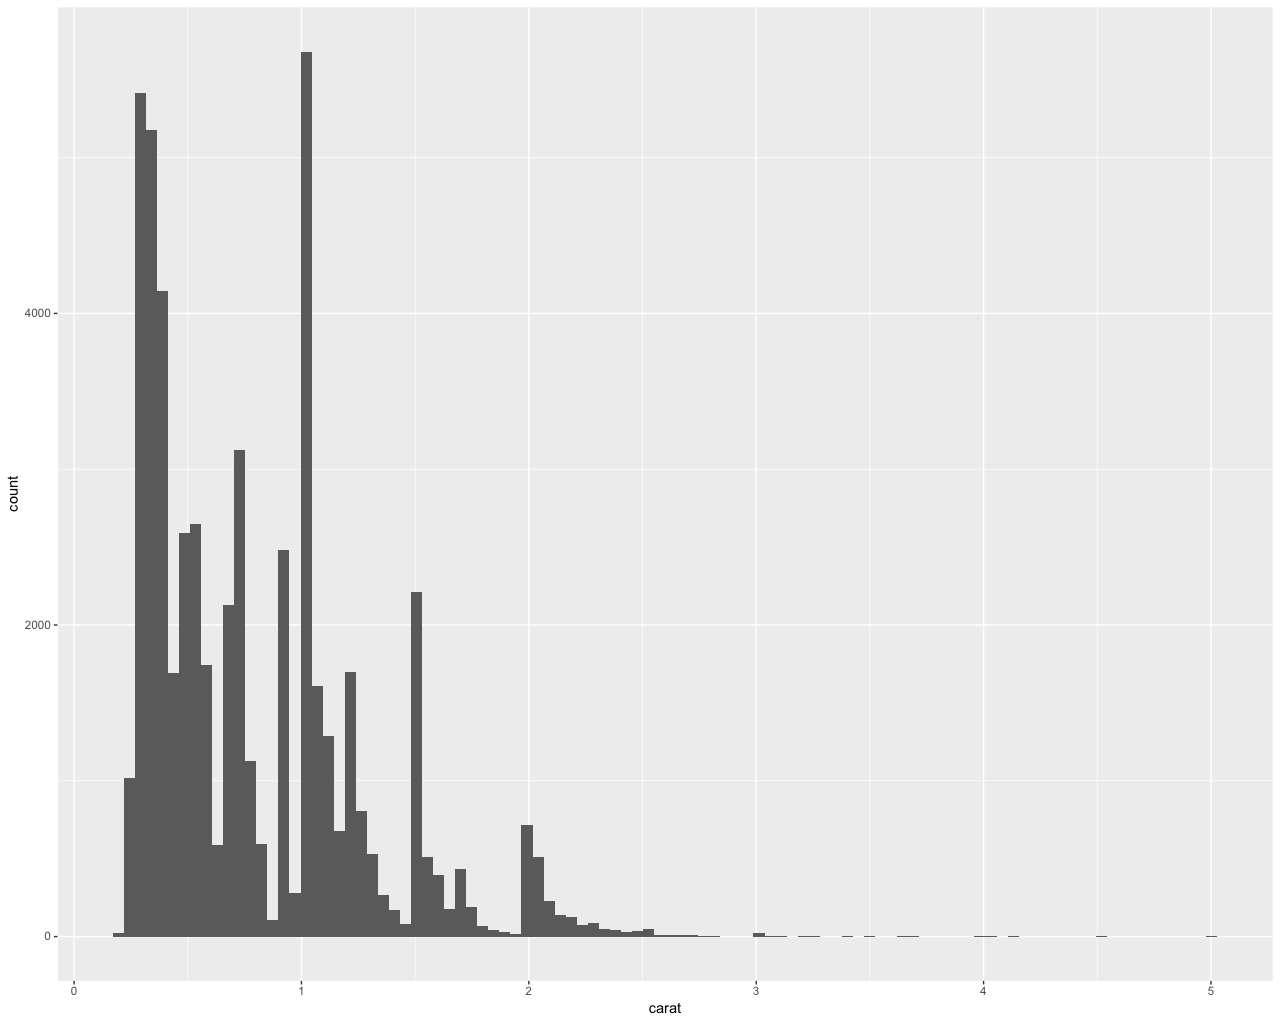
\includegraphics[width=1.0\linewidth]{pic0031}
  \caption{Хистограма при 100 групи}
\label{figure0031}
\end{figure}
\FloatBarrier

Размерът на групите в хистограмата може да варира (Фиг. \ref{figure0030},\ref{figure0031}). За да се изчертае плътностна функция е достатъчно графичният обект, генериран от ggplot, да бъде декориран с функцията geom\_density (Фиг. \ref{figure0032}), вместо с функцията geom\_histogram. 


\begin{figure}[h!]
  \centering
  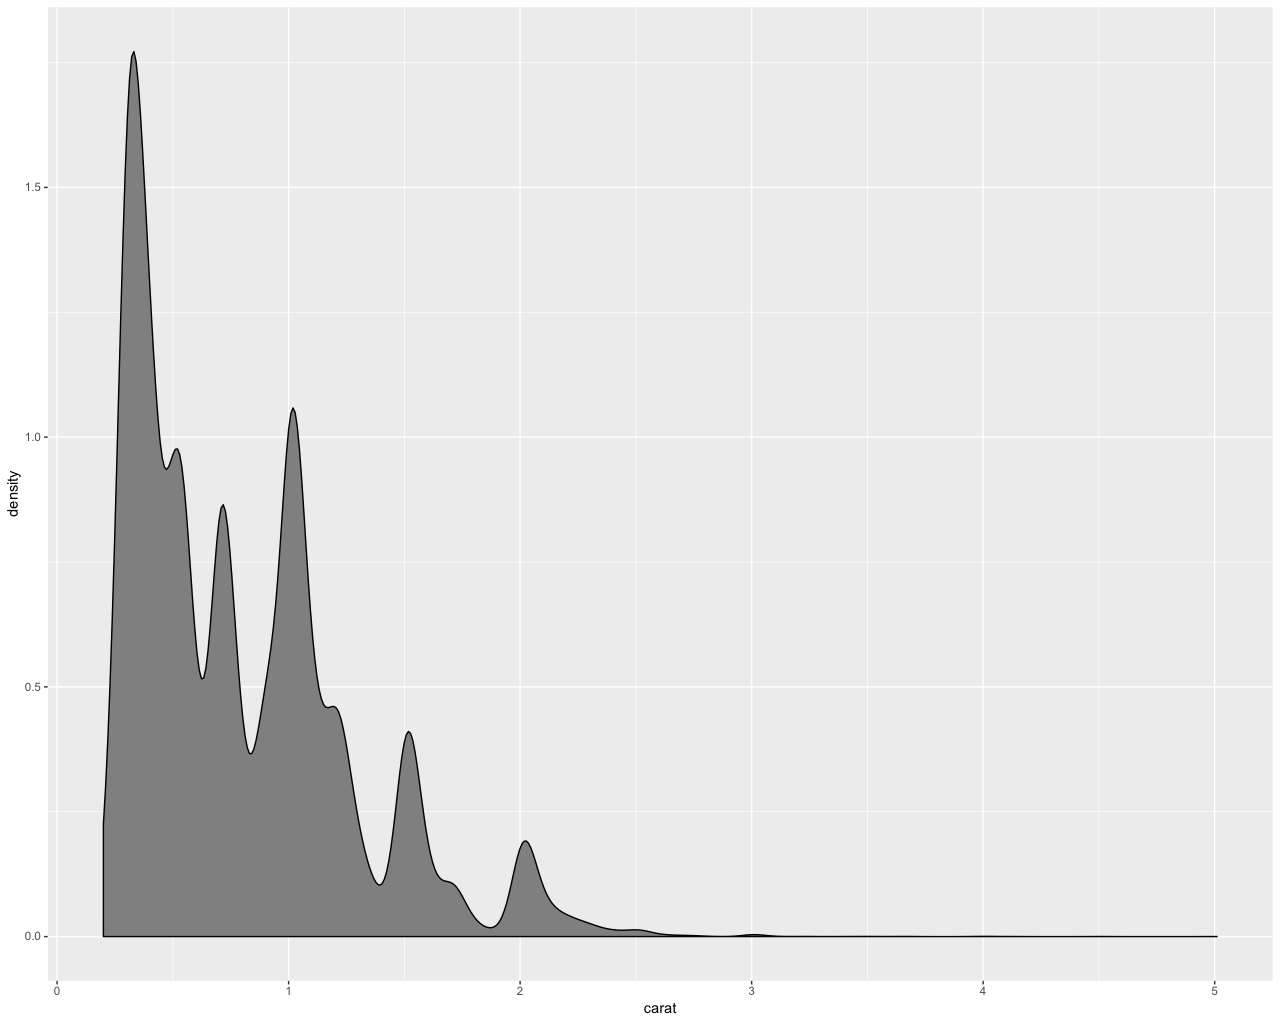
\includegraphics[width=1.0\linewidth]{pic0032}
  \caption{Плътностна функция}
\label{figure0032}
\end{figure}
\FloatBarrier

Хистограмата показва броене по групи, докато плътностната функция задава вероятността определен камък да попадне в предварително определен интервал. Макар и много да си приличат, хистограмата и плътностната функция са подходящи в два различни случая. Хистограмите са полезни при дискретни случайни величини, докато плътностните функции намират повече употреба в непрекъснатите случайни величини. 

\subsection{Диаграми на разсейване}

\section*{Заключение}

